%导言区
\documentclass{article}

\usepackage{ctex}
\title{深度学习目标检测}
\date{\today}

\usepackage[a4paper,left=10mm,right=10mm,top=15mm,bottom=15mm]{geometry} 
\usepackage{listings}
\setlength{\parindent}{0pt}% 去掉首行缩进。
\usepackage{titlesec}
%\usepackage[center]{titlesec}%设置标题格式。
%\titleformat{\section}{\centering}
%\titleformat{\section}{\centering\Huge\bfseries}{第\,\thechapter\,章}{1em}{}
\usepackage{graphicx}
\begin{document}
	\maketitle
	\begin{abstract}
		计算机视觉研究中,目标检测是一个比分类更困难的领域,我们将回顾它的历史和最近的发展。在深度学习时代之前,像 HOG 和特征金字塔这样的手工特性被广泛用于获取图像中的定位信号。然而,这些方法通常不能很好地扩展到通用的目标检测,所以大多数的应用仅限于人脸识别或者行人检测。利用深度学习的力量,我们可以训练一个网络来学习要获取的特征,并预测目标的坐标。这最终带来了基于视觉感知的应用的繁荣,比如商业人脸识别系统和无人机。在这篇文章里,我为那些想要学习目标检测的新手挑选了12篇必读论文。尽管构建目标检测系统最具挑战性的部分隐藏在实现细节中,但是阅读这些论文仍然可以让你对这些想法的来源以及未来目标检测将如何发展有一个很好的大致理解。
		作为阅读本文的前提条件,你需要了解卷积神经网络的基本思想,以及常用的优化方法,如带反向传播的梯度下降法。还有图像分类的基础知识,因为目标检测的许多很酷的想法都来源于更基础的图像分类研究。
		\begin{quotation}
		\noindent https://towardsdatascience.com/
		12-papers-you-should-read-to-understand-object-detection-in-the-deep-
		learning-era-3390d4a28891
		\end{quotation}
		
	\end{abstract}
	
	   	\section{2013:OverFeat} 
	   	OverFeat: Integrated Recognition, Localization and Detection using Convolutional Networks
	   	
	   	在2012年的 ImageNet 竞赛中,基于 CNN 特征提取的AlexNet击败了所有手工设计的特征提取器。受到 AlexNet 成功的启发,OverFeat 迅速将 CNN 引入到目标检测领域。这个想法非常直接: 如果我们可以用 CNN 对一张图片进行分类,那么用不同大小的窗口滑动浏览整张图片,然后尝试用 CNN 逐一对它们进行分类呢?该算法利用了 CNN 的特征提取和分类能力,并通过预定义的滑动窗口绕过了硬 region proposal 问题。另外,由于邻近的卷积核可以共享部分计算结果,因此不需要计算重叠区域的卷积,从而大大降低了成本。OverFeat 是单阶段目标检测器的先驱。它试图在同一个 CNN 中结合特征提取、位置回归和区域分类。不幸的是,这种单阶段的方法由于使用较少的先验知识,精确度也相对较差。因此,OverFeat 未能引领单阶段检测器研究的热潮,直到两年后出现了一个更优雅的解决方案。
	   	
	   	在上图中,R-CNN 首先使用一种称为selective search的技术从输入图像中提取出感兴趣的潜在区域。selective search并不真正尝试理解前景目标,相反,它依靠启发式方法对相似的像素进行分组: 相似的像素通常属于同一个目标。因此,selective search的结果很有可能包含一些有意义的内容。接下来,R-CNN 将这些 region proposals 变换成带有一些填充的固定大小的图像,并将这些图像提供给网络的第二阶段,以便进行更细粒度的识别。与那些使用selective search的旧方法不同,R-CNN 在第二阶段将 HOG 替换为 CNN,从所有 region proposals 中提取特征。这种方法需要注意的是,许多 region proposals 实际上并不是一个完整的目标,因此 R-CNN 不仅需要学习如何对包含的类别进行分类,还需要学习如何拒绝负类。为了解决这个问题,R-CNN 将所有与一个ground truth框重叠度≥0.5 IoU 的 region proposal 视为正,其余视为负。
	   	selective search 的 region proposal 高度依赖于相似性假设,因此只能提供大致的位置估计。为了进一步提高定位精度,R-CNN 借鉴了“Deep Neural Networks for Object Detection”(又名 DetectorNet)的思想,引入了额外的边界框回归来预测框的中心坐标、宽度和高度。这种回归器被广泛应用于未来的目标检测器中。
	   	然而,像 R-CNN 这样的两阶段检测器存在两个大问题: 1) selective search并不是卷积,因为它不是端到端可训练的。2) region proposal 阶段与 OverFeat 等其他单阶段检测器相比通常非常慢,而且在每个 region proposal上分别运行会使其更慢。稍后,我们将看到 R-CNN 如何随着时间的推移逐步演变以解决这两个问题的。
	   	
	   	\section{R-CNN基于区域卷积网络的精确目标检测和分割}
	   R-CNN 也是在2013年提出的,比 OverFeat 晚了点。然而,这种基于区域的方法最终以其两阶段的框架,即 region proposal 阶段和区域分类与精细化阶段,引发了目标检测研究的大浪潮。
	   
	   \begin{figure}[htpb]
	   	\centering
	   	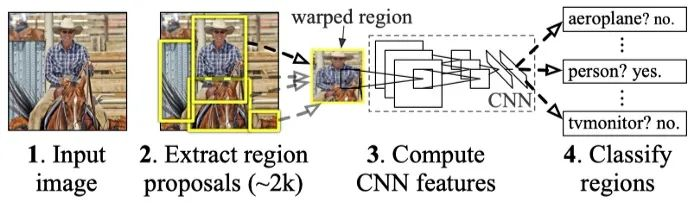
\includegraphics[width=\linewidth]{detectfig/1.jpg}
	   	\caption{源自论文“Region-based Convolutional Networks for Accurate Object Detection and Segmentation”}
	   \end{figure}
	   在上图中,R-CNN 首先使用一种称为selective search的技术从输入图像中提取出感兴趣的潜在区域。selective search并不真正尝试理解前景目标,相反,它依靠启发式方法对相似的像素进行分组: 相似的像素通常属于同一个目标。因此,selective search的结果很有可能包含一些有意义的内容。接下来,R-CNN 将这些 region proposals 变换成带有一些填充的固定大小的图像,并将这些图像提供给网络的第二阶段,以便进行更细粒度的识别。与那些使用selective search的旧方法不同,R-CNN 在第二阶段将 HOG 替换为 CNN,从所有 region proposals 中提取特征。这种方法需要注意的是,许多 region proposals 实际上并不是一个完整的目标,因此 R-CNN 不仅需要学习如何对包含的类别进行分类,还需要学习如何拒绝负类。为了解决这个问题,R-CNN 将所有与一个ground truth框重叠度≥0.5 IoU 的 region proposal 视为正,其余视为负。
	   selective search 的 region proposal 高度依赖于相似性假设,因此只能提供大致的位置估计。为了进一步提高定位精度,R-CNN 借鉴了“Deep Neural Networks for Object Detection”(又名 DetectorNet)的思想,引入了额外的边界框回归来预测框的中心坐标、宽度和高度。这种回归器被广泛应用于未来的目标检测器中。
	   然而,像 R-CNN 这样的两阶段检测器存在两个大问题: 1) selective search并不是卷积,因为它不是端到端可训练的。2) region proposal 阶段与 OverFeat 等其他单阶段检测器相比通常非常慢,而且在每个 region proposal上分别运行会使其更慢。稍后,我们将看到 R-CNN 如何随着时间的推移逐步演变以解决这两个问题的。
	   	
	   	\section{2015: Fast R-CNN}
	   	R-CNN 的一个快速后续是减少对多个 region proposals 的重复卷积。由于这些 region proposals 都来自一个图像,自然而然地想到,可以通过对整个图像运行一次 CNN,并在许多 region proposals 之间共享计算,来改进 R-CNN。然而,不同的 region proposals 有不同的大小,如果我们使用相同的 CNN 特征提取器,会导致不同的输出特征图大小。这些具有不同大小的特征图将阻止我们使用全连接层进行进一步的分类和回归,因为全连接层的输入只能是固定大小。
	   	
	   	\begin{figure}[htpb]
	   		\centering
	   		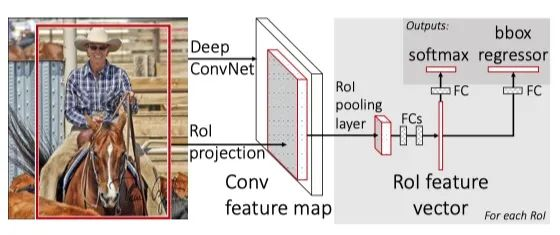
\includegraphics[width=\linewidth]{detectfig/2.jpg}
	   		\caption{源自论文“Fast R-CNN”}
	   	\end{figure}
	   	幸运的是,论文“Spatial Pyramid Pooling in Deep Convolutional Networks for Visual Recognition”解决了全连接层的动态缩放问题。在 SPPNet 中,在卷积层和 FC 层之间引入了特征金字塔池化,以创建bag-of-words式的特征向量。这个向量有固定的大小和不同尺度的特征特征,所以我们的卷积层现在可以接受任意尺寸的图像作为输入,而不用担心 FC 层的不兼容性。受此启发,Fast R-CNN 提出了一个类似的层称为 ROI Pooling 层。这个池化层将不同大小的特征图 downsample 为一个固定大小的向量。这样我们就可以使用相同的 FC 层进行分类和框回归,不管 ROI 是大还是小。
	   	
	   	Fast R-CNN 由于采用了共享特征提取器和尺度不变(scale-invariant)的 ROI 池化层,达到类似的定位精度,训练快了10 ~ 20倍,且推理快了100 ~ 200倍。接近实时推理和一个更易用的端到端检测部分训练协议使Fast R-CNN 成为业界的热门选择。
	   	
	   	\section{2015: Faster R-CNN 通过Region Proposal Networks实现实时目标检测}
	   	正如我们上面介绍的,在2015年初,Ross Girshick 提出了一个改进版本的 R-CNN,称为 Fast R-CNN,对建议的区域使用共享的特征提取器。仅仅几个月后,Ross和他的团队又带着另一个改进回来了。这个新的网络Faster R-CNN 不仅比以前的版本更快,而且标志着目标检测深度学习方法的一个里程碑。
	   	
	   	\begin{figure}[htpb]
	   		\centering
	   		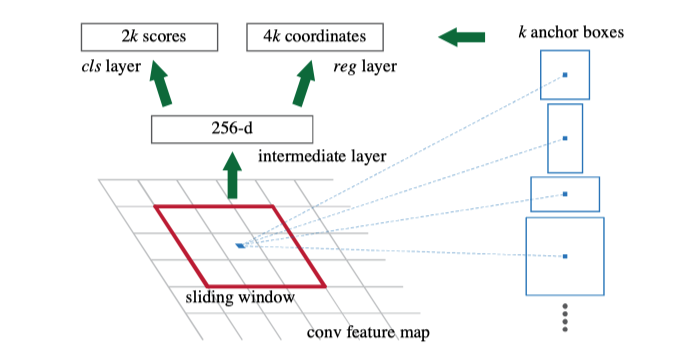
\includegraphics[width=\linewidth]{detectfig/3.png}
	   		\caption{源自论文“Faster R-CNN: Towards Real-Time Object Detection with Region Proposal Networks”}
	   	\end{figure}
   	
	   	有了 Fast R-CNN,网络中唯一的非卷积部分就是 selective search 的 region proposal了。2015年,研究人员开始意识到深层神经网络是如此神奇,只要有足够的数据,它就可以学习任何东西。那么,是否有可能训练一个 region proposal 的神经网络,而不是依赖于 selective search 等启发式和手工的方法?Faster R-CNN 遵循这个方向和思路,并成功地创建了Region Proposal Network(RPN)。简单地说,RPN 是一个 CNN,以图像作为输入,并输出一组矩形目标建议,每个都有一个 objectiveness 得分。论文最初使用的是 VGG,但其他主干网络如 ResNet 后来变得更加普及。为了生成 region proposals,在 CNN 特征图输出上应用一个3x3滑动窗口每个位置生成2个得分(前景和背景)和4个坐标值。实际上,这个滑动窗口是用一个带有1x1卷积核的3x3卷积核来实现的。
	   	
	   	\begin{figure}[htpb]
	   		\centering
	   		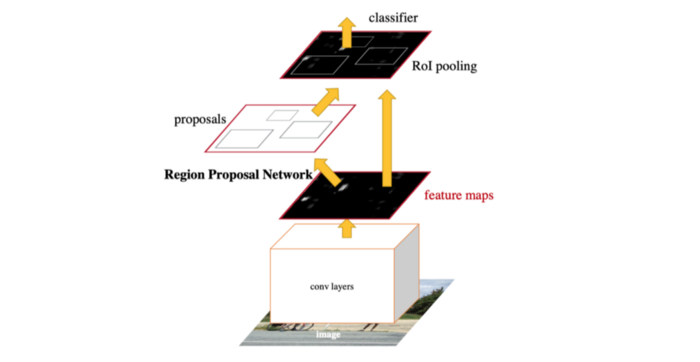
\includegraphics[width=\linewidth]{detectfig/4.png}
	   		\caption{源自论文“Faster R-CNN: Towards Real-Time Object Detection with Region Proposal Networks”ss}
	   	\end{figure}
   	
	   	虽然滑动窗口有一个固定的大小,我们的目标可能有不同的尺度。因此,Faster R-CNN 引入了一种称为 anchor box 的技术。Anchor boxes 是预先定义的具有不同宽高比和尺寸的框,但共享相同的中心位置。在 Faster R-CNN 中,每个滑动窗口位置都有 k = 9个anchors,每个anchor 覆盖3个高宽比和3个尺度。这些不同尺度的重复 anchor boxes 在共享同一特征图输出的同时,为网络带来了良好的平移不变性和比例不变性。请注意,边界框回归将从这些anchor box 而不是从整个图来计算。
	   	
	   	到目前为止,我们讨论了新的 Region Proposal Network 来取代旧的 selective search 进行region proposal。为了进行最终的检测,Faster R-CNN 使用与 Fast R-CNN 相同的检测头进行分类和细粒度定位。你还记得 Fast R-CNN 还使用共享的 CNN 特性提取器吗?既然 RPN 本身也是一个特征提取 CNN,我们可以像上面的图表那样与检测头共享它。这种分享设计并不会带来什么麻烦。如果我们一起训练 RPN 和 Fast R-CNN 检测器,我们将把 RPN proposals 作为 ROI 池化的一个常量输入,并且不可避免地忽略 RPN 边界框proposals的梯度。一个绕开方法被称为替代训练,即轮流训练 RPN 和Fast R-CNN 。在后来的论文“Instance-aware semantic segmentation via multi-task network cascades”中,我们可以看到 ROI 池化层也可以对框坐标proposals微分。
	   	
	   	\section{2015: YOLO v1}
	   	虽然 R-CNN 系列在研究界引起了关于两阶段目标检测的大肆炒作,但其复杂的实现给维护它的工程师们带来了许多头疼的问题。目标检测有必要这么麻烦吗?如果我们愿意牺牲一点准确率,我们能换来更快的速度吗?带着这些问题,Joseph Redmon 在 Faster R-CNN 发布仅仅四天后就向http://arxiv.org提交了一个名为 YOLO 的网络,并且在 OverFeat 首次亮相两年后,终于将人气带回到了单阶段目标检测。
	   	
	   	\begin{figure}[htpb]
	   		\centering
	   		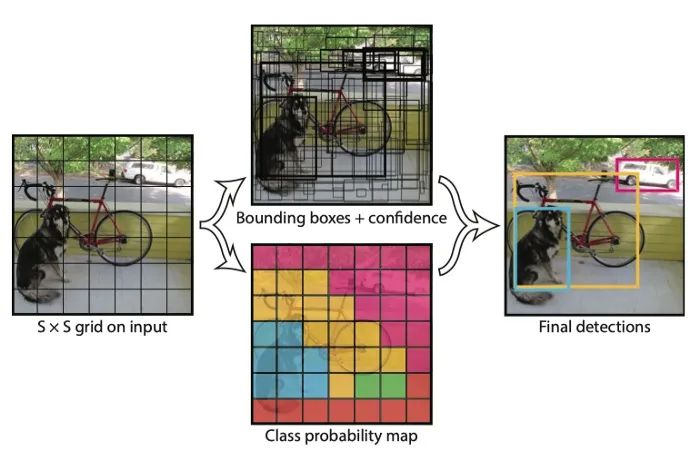
\includegraphics[width=\linewidth]{detectfig/5.jpg}
	   		\caption{源自论文“You Only Look Once: Unified, Real-Time Object Detection”}
	   	\end{figure}
%	   	{源自论文“You Only Look Once: Unified, Real-Time Object Detection”}
	   	
	   	与 R-CNN 不同的是,YOLO 决定在同一个 CNN 上一起处理region proposal和分类。换句话说,它把目标检测问题看作是一个回归问题,而不是一个依赖于region proposal的分类问题。其基本思想是将输入分割成一个 SxS 网格,并让每个单元直接回归边界框的位置以及如果目标中心落入该单元时的置信度得分。因为目标可能有不同的大小,将有一个以上的边界框回归器落到每个单元。在训练过程中,将指定IOU最高的回归器与ground-truth 标签进行比较,因此同一位置的回归器将学会随着时间的推移处理不同的尺度。同时,当网格单元包含一个目标(高置信度得分)时,每个单元也将预测 C 类概率。这种方法后来被描述为稠密的预测,因为 YOLO 试图预测图像中所有可能位置的类和边界框。相比之下,R-CNN 依赖于region proposals来过滤背景区域,因此最终的预测更加稀疏。
	   	
	   	\begin{figure}[htpb]
	   		\centering
	   		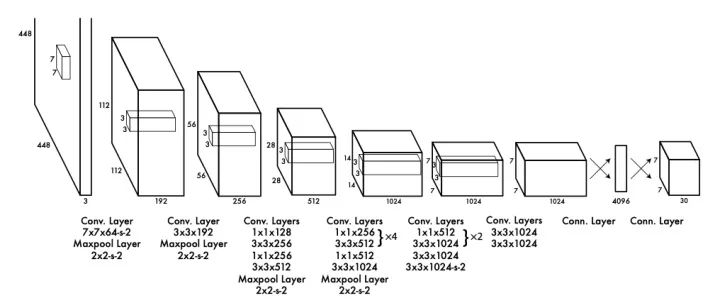
\includegraphics[width=\linewidth]{detectfig/6.jpg}
	   		\caption{源自论文“You Only Look Once: Unified, Real-Time Object Detection”ss}
	   	\end{figure}
	   	
	   	
	   	在整张图片上的密集预测的计算成本很大,为了避免这个问题,YOLO 采用了 GooLeNet 的瓶颈结构。YOLO 的另一个问题是,两个对象可能落入同一个粗糙的网格单元,所以它不能很好地处理小目标,如一群鸟。尽管精确度较低,但 YOLO 简单易懂的设计和实时推理能力使得单阶段目标检测在研究中再次流行起来,同时也是业界的首选解决方案。
	   	
	   	\section{2015: SSD  单发多框检测器} 
	   	YOLO v1显示了单阶段检测的潜力,但和两阶段检测的性能差距仍然很明显。在 YOLO v1中,可以将多个目标分配给同一个网格单元。这对于探测微小物体来说是一个巨大的挑战,也成为提高单阶段检测器性能到与两阶段检测器相当的关键问题。SSD是一个挑战者,从三个角度解决这个问题。
	   	
	   	\begin{figure}[htpb]
	   		\centering
	   		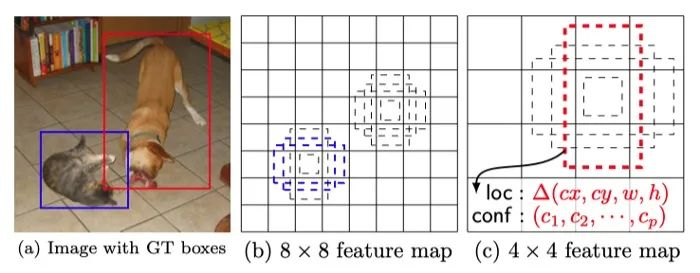
\includegraphics[width=\linewidth]{detectfig/7.jpg}
	   		\caption{源自论文 “SSD: Single Shot MultiBox Detector”}
	   	\end{figure}
   	
	   	首先,来自 Faster R-CNN 的anchor box 技术可以缓解这个问题。同一区域中的对象通常具有不同的可见长宽比。引入anchor box 不仅增加了每个单元的目标检测数量,而且利用这个长宽比假设可以更好地区分重叠的小目标。
	   	
	   	\begin{figure}[htpb]
	   		\centering
	   		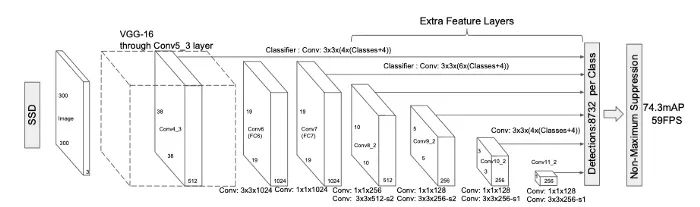
\includegraphics[width=\linewidth]{detectfig/8.jpg}
	   		\caption{源自论文 “SSD: Single Shot MultiBox Detector”ss}
	   	\end{figure}
   	
	   	SSD 进一步在检测之前聚合多尺度特征。这是一个提取细粒度的局部特征非常常见的方法,同时保留粗糙的全局特征在 CNN 中。例如,CNN 语义分割的先驱 FCN 也从多个层次对特征进行融合,以提取分割的边界。此外,多尺度特征聚合可以方便地在所有常用的分类网络上进行,从而方便了主干网与其他网络的替换。
	   	最后,SSD 利用了大量的数据增强,特别是针对小目标。例如,在随机裁剪之前,图像被随机扩展到更大的尺寸,这给训练数据带来了缩放效果,以模拟小目标。此外,大的边界框通常很容易学习。为了避免这些简单的样本主导损失函数,SSD 采用了一种hard negative mining技术,为每个anchor box选出损失最大的样本。
	   	
	   	
	   	
	   	\section{2016: FPN 目标检测的特色金字塔网络} 
	   	随着 Faster-RCNN、 YOLO 和 SSD 在2015年的发布,似乎确定了目标检测器的总体结构。研究人员开始着眼于改善这些网络的每个单独部分。特征金字塔网络是利用不同层次的特征构成特征金字塔,从而改进检测头的一种尝试。这种特征金字塔的想法在计算机视觉研究中并不新奇。当特征还是手工设计的时候,特征金字塔已经是识别不同尺度模式的一种非常有效的方法。在深度学习中使用特征金字塔也不是一个新的想法: SSPNet、 FCN 和 SSD 都证明了在分类之前聚合多层特征的好处。然而,如何在 RPN 和基于区域的检测器之间共享特征金字塔仍然有待于确认。
	   	
	   	\begin{figure}[htpb]
	   		\centering
	   		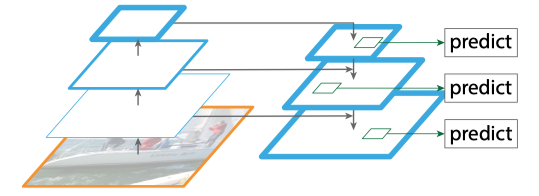
\includegraphics[width=\linewidth]{detectfig/9.png}
	   		\caption{源自论文 “Feature Pyramid Networks for Object Detection”}
	   	\end{figure}
   	
	   	首先,为了使用如上图所示的 FPN 结构重新构建 RPN,我们需要有一个在多个不同尺度的特征输出上运行的region proposal。此外,我们现在每个位置只需要3个不同长宽比的anchors,因为不同大小的物体将由不同层次的特征金字塔处理。接下来,为了在 Fast R-CNN 检测器中使用 FPN 结构,我们还需要对其进行改造,以便在多种尺度的特征图上进行检测。由于region proposals也可能有不同的尺度,我们也应该在 FPN 的相应层级上使用它们。简而言之,如果Faster R-CNN 是一对运行在一个尺度上的 RPN 和基于区域的检测器,FPN 将其转换成在不同尺度上运行的多个并行分支,并最终从所有分支中收集最终结果。
	   	
	   	\section{2016: YOLO v2 9000} 
	   	当何凯明、Ross Girshick和他们的团队不断改进他们的两阶段 R-CNN 探测器时,另一边,约Joseph Redmon也在忙于改进他的单阶段 YOLO 检测器。最初版本的 YOLO 存在许多缺点: 基于粗网格的预测带来了较低的定位精度,每个网格单元有两个尺度不确定的回归器也使得识别小目标变得困难。幸运的是,2015年我们在许多计算机视觉领域看到了太多伟大的创新。YOLO v2只是需要找到一种方法来整合它们,使它们变得更好、更快、更强。以下是修改的一些亮点:
	   	
	   	YOLO v2增加了一个Batch Normalization层,这个层来自论文“Batch Normalization: Accelerating Deep Network Training by Reducing Internal Covariate Shift”。
	   	
	   	\begin{figure}[htpb]
	   		\centering
	   		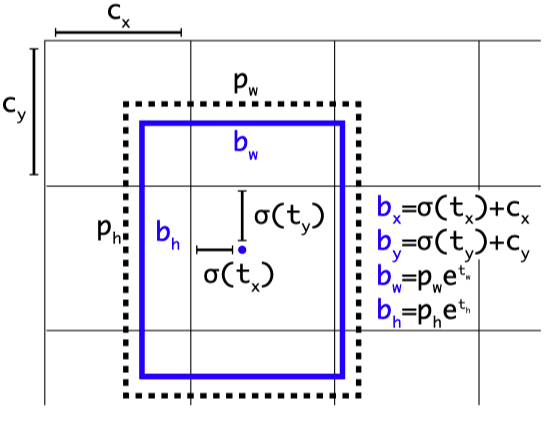
\includegraphics[width=\linewidth]{detectfig/10.png}
	   		\caption{Anchor boxes,源自论文“YOLO9000: Better, Faster, Stronger”}
	   	\end{figure}
	   	
	   	就像 SSD 一样,YOLO v2也引入了 Faster R-CNN 用于边界框回归的anchor boxes思想。但是 YOLO v 2为它的anchor boxes做了一些定制。YOLOv2不是预测anchor boxes的偏移量,而是约束目标中心回归tx 和ty,限制在负责的网格单元内,以稳定早期训练。此外,anchors的大小是由目标数据集的 K-means聚类算法来决定的,以便更好地与目标形状对齐。
	   	
	   	
	   	一个名为 Darknet 的新主干网用于特征提取。受到“Network in Network” 和GooLeNet’的瓶颈结构启发。
	   	为了改进对小目标的检测,YOLO v2增加了一个passthrough层来合并早期层的特征。这部分可以看作是 SSD 的简化版。
	   	
	   	最后但并非最不重要的一点是,Joseph 意识到输入分辨率对于小目标检测来说是一颗银弹。它不仅将主干的输入从224x224增加到448x448,而且还发明了一种多尺度的训练方案,其中涉及到在不同的训练阶段使用不同的输入分辨率。
	   	
	   	注意,YOLO v2还试验了一个版本,该版本在9000个类的分层数据集上训练,这也代表了目标检测器中多标签分类的早期试验。
	   	
	   	
	   	\section{2017: RetinaNet 针对密集目标检测的Focal Loss} 
	   	为了理解为什么单阶段检测器通常不如两阶段检测器好,RetinaNet 研究了单阶段检测器密集预测的前景-背景类不均衡问题。以 YOLO 为例,它试图同时预测所有可能位置的类和边界框,因此在训练过程中大多数输出与负类相匹配。SSD 通过 hard example mining解决了这个问题。在训练的早期阶段,YOLO 使用objectiveness评分隐式训练前景分类器。RetinaNet认为他们都没有找到解决问题的关键,所以它发明了一种新的损失函数,称为Focal Loss,以帮助网络学习什么是真正重要的。
	   	
	   	$$\mathrm{FL}\left(p_{\mathrm{t}}\right)=-\alpha_{\mathrm{t}}\left(1-p_{\mathrm{t}}\right)^{\gamma} \log \left(p_{\mathrm{t}}\right)$$
	   	
	   	源自论文“Focal Loss for Dense Object Detection”
	   	
	   	Focal Loss 增加了一个指数 γ (他们称之为聚焦参数)的交叉熵损失。自然,随着置信度分数的增加,损失值会比正常的交叉熵值低得多。参数 α 用于平衡这种聚焦效应。
	   	
	   	\begin{figure}[htpb]
	   		\centering
	   		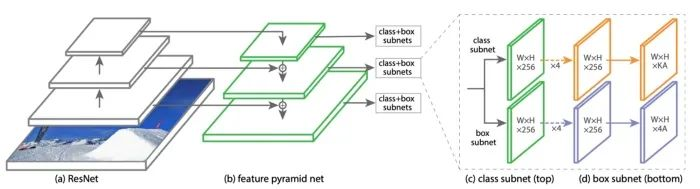
\includegraphics[width=\linewidth]{detectfig/11.jpg}
	   		\caption{源自论文“Focal Loss for Dense Object Detection”}
	   	\end{figure}
	   	
	   	这个想法很简单,即使是小学生也能理解。为了进一步证明他们的工作,他们调整了之前提出的 FPN 模型,并创建了一个新的单阶段检测器,称为 RetinaNet。它由 ResNet 主干网、不同尺度信道特征的 FPN 检测颈、作为检测头的分类子网和框回归子网组成。类似于 SSD 和 YOLO v3,RetinaNet 使用anchor boxes 覆盖不同尺度和长宽比的目标。
	   	
	   	稍微离题一下,RetinaNet 使用了 ResNeXT-101和800输入分辨率的 COCO 精确度来对比 YOLO v2,而YOLO v2只有一个轻量的 Darknet-19主干和448输入分辨率。这种不真诚表明团队强调获得的更好的基准测试结果,而不是解决像速度准确性 trade-off这样的实际问题。这可能是 RetinaNet 发布后没有起飞的部分原因。
	   	
	   	
	   	\section{2018: YOLOv3: 渐进式改进} 
	   	
	   YOLO v3 是官方 YOLO 系列的最后一个版本。遵循 YOLO v2的传统,YOLO v3从以前的研究中借鉴了更多的想法,并且得到了一个难以置信的像怪物一样强大的单阶段检测器。YOLO v3很好地平衡了速度、准确率和实现的复杂性。由于它的快速和简单的组件,它在行业中非常受欢迎。
	  
	  \begin{figure}[htpb]
	  	\centering
	  	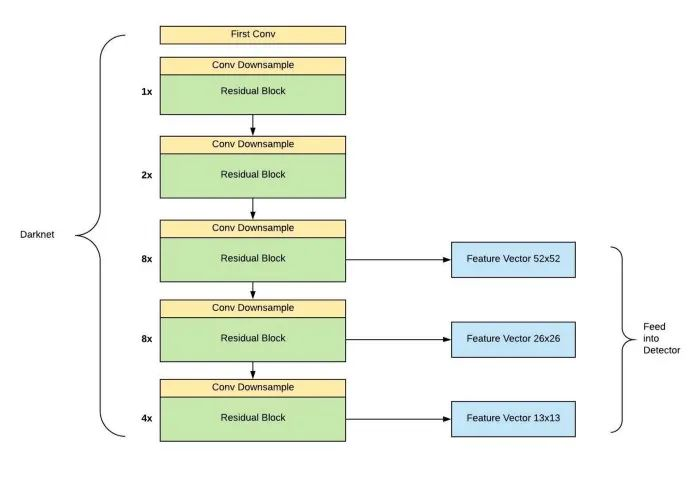
\includegraphics[width=\linewidth]{detectfig/12.jpg}
	  	\caption{源自论文“Dive Really Deep into YOLO v3: A Beginner’s Guide”}
	  \end{figure}
  \begin{figure}[htpb]
  	\centering
  	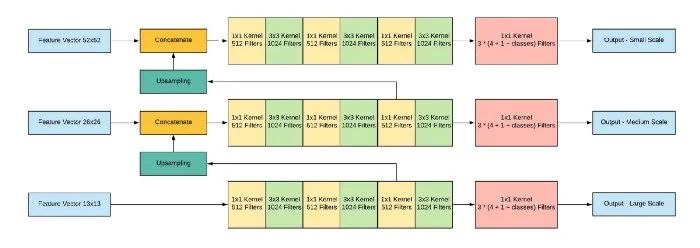
\includegraphics[width=\linewidth]{detectfig/13.jpg}
  	\caption{源自论文“Dive Really Deep into YOLO v3: A Beginner’s Guide”ss}
  \end{figure}
	  
	  简单地说,YOLO v3的成功来自于它更强大的主干功能提取器和带有 FPN 颈部的类似 RetinaNet 的检测头。新的主干网络 Darknet-53利用了 ResNet 的skip连接,以达到与 ResNet-50相当的准确度,但速度要快得多。此外,YOLO v3抛弃了 v2的pass through层,完全采用 FPN 的多尺度预测设计。从那时起,YOLO v3终于扭转了人们对它在处理小目标时表现不佳的印象。
	  
	  此外,关于 YOLO v3还有一些有趣的事实。它diss了 COCO mAP 0.5:0.95度量标准,证明了条件密集预测时Focal Loss没啥用。一年后作者Joseph甚至决定放弃整个计算机视觉研究,因为他担心会用到军事上。
	 
	\section{2019: Objects As Points}
	尽管近年来图像分类领域变得不那么活跃,但目标检测的研究还远未成熟。2018年,一篇名为“CornerNet: Detecting Objects as Paired Keypoints””的论文为检测器训练提供了一个新的视角。由于准备anchor box目标是一个相当繁琐的工作,是否真的有必要使用他们作为先决条件?这种抛弃 anchor boxes的新趋势被称为“anchor-free”目标检测。
	
	受Hourglass网络中热图用于人体姿态估计的启发,CornerNet 使用框角生成的热图来监督边界框回归。
	
	
	\begin{figure}[htpb]
		\centering
		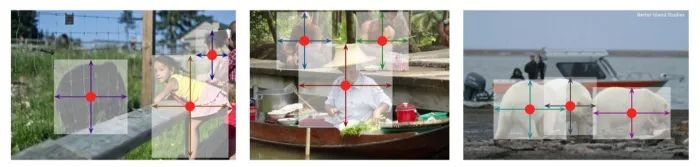
\includegraphics[width=\linewidth]{detectfig/14.jpg}
		\caption{源自论文“Objects as Points”}	
	\end{figure}

	Objects As Points,又名 CenterNet,更进了一步。它使用热图峰值来表示物体中心,网络将直接从这些框中心回归框的宽度和高度。实际上,CenterNet 使用每个像素作为网格单元。使用高斯分布的热图,与之前直接回归边界框大小的尝试相比,训练也比较容易收敛。
	
	消除anchor boxes还有另一个有用的副作用。以前,我们依赖anchor boxe和ground truth框之间的IOU(如 > 0.7)来分配训练目标。这样一些相邻的anchors都被分配了同一个目标的正目标。网络也将学会为同一个物体预测多个正框。解决这个问题的常用方法是使用一种称为非极大值抑制(Non-maximum Suppression,NMS)的技术。这是一个贪婪算法,过滤掉太靠近的框。现在anchors消失了,我们在热图中每个目标只有一个峰值,不再需要使用 NMS 了。由于 NMS 有时难以实现且运行缓慢,因此对于在资源有限的各种环境中运行的应用程序来说,摆脱 NMS 是一个很大的好处。
	
	\section{2019: EfficientDet 可扩展和高效的目标检测}
	
	在最近的 CVPR’20中,EfficientDet 向我们展示了目标检测领域更令人兴奋的发展。FPN 结构已被证明是提高检测网络在不同尺度下对目标检测性能的有力技术。著名的检测网络,如 RetinaNet 和 YOLO v3,在框回归和分类之前都采用了 FPN 颈。后来,NAS-FPN 和 PANet (请参阅阅读更多部分)都证明了一个普通的多层 FPN 结构可能会受益于更多的设计优化。EfficientDet继续朝这个方向探索,最终创造了一个新的脖,叫做 BiFPN。基本上,BiFPN 提供了额外的跨层连接,以鼓励来回的特性聚合。为了证明网络的效率,BiFPN 从原始的PANet设计中删除了一些不太有用的连接。FPN 结构上的另一个创新改进是权重特征融合。BiFPN 增加了额外的可学习的权重来实现聚合,这样网络就可以学习不同分支的重要性。
	
	\begin{figure}[htpb]
		\centering
		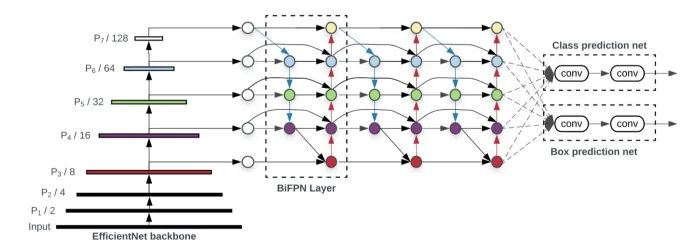
\includegraphics[width=\linewidth]{detectfig/15.jpg}
		\caption{源自论文“EfficientDet: Scalable and Efficient Object Detection”}
	\end{figure}
\begin{figure}[htpb]
	\centering
	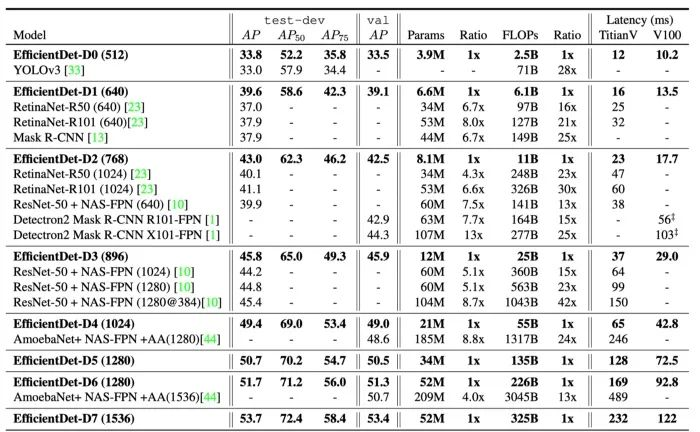
\includegraphics[width=\linewidth]{detectfig/16.jpg}
	\caption{源自论文“EfficientDet: Scalable and Efficient Object Detection”ss}
\end{figure}
	
	此外,就像我们在图像分类网络 EfficientNet 中看到的一样,EfficientDet 也引入了一种合理的方法来缩放目标检测网络。上述公式中的参数φ 同时控制了 BiFPN 颈部和检测头的宽度(通道)和深度(层)。
	
	这个新参数产生了8个不同的 EfficientDet 变种,从 D0到 D7。一个轻量级的 D0变种可以达到与 YOLO v3相似的精度,而FLOPs更少。一个重型的 D7变种,加上可怕的1536x1536输入,甚至在 COCO 上可以达到53.7 AP ,使所有其他竞争者相形见绌。
	
	\section{相关组件发展}
	\subsection{2009: DPM}
	
	基于分离部分训练的目标检测模型
	通过为每个可变形的部件匹配很多 HOG 特征,DPM 是深度学习时代之前最有效的目标检测模型之一。以行人检测为例,首先采用星型结构识别通用人模式,然后用不同的子滤波器识别各部分并计算总分。即使在今天,在我们从 HOG 特征转换到 CNN 特征之后,通过各个可变形部件来识别目标的想法仍然很流行。
	2012: Selective Search
	
	\subsection{物体识别的Selective Search}
	和 DPM 一样,Selective Search 也不是深度学习时代的产物。然而,这种方法将许多经典的计算机视觉方法结合在一起,也用于早期的 R-CNN 检测器。selective search的核心思想来自于语义分割,即通过相似度对像素进行分组。selective search使用不同的相似度标准,如颜色空间和基于 SIFT 的纹理来迭代合并相似的区域在一起。这些合并后的区域用作前景预测,然后用支持向量机分类器进行目标识别。
	2016: R-FCN
	
	\subsection{R-FCN: 通过基于区域的全卷积网络实现目标检测}
	Faster R-CNN 最终结合了 RPN 和 ROI 特征提取,大大提高了速度。然而,对于每个region proposal,我们仍然需要全连接层来分别计算类和边界框。如果有300个 ROIs,我们需要重复300次,这也是单阶段和两阶段检测器之间速度差异的主要原因。R-FCN 借鉴了 FCN 语义分割的思想,但是 R-FCN 没有计算类掩码,而是计算了一个正敏感的得分图。这张图将预测物体在每个位置出现的概率,并且所有位置将投票(平均)来决定最终的类和边界框。此外,R-FCN 还在其 ResNet 主干中使用了 atrous 卷积,这种卷积最初是在 DeepLab 语义分割网络中提出的。
	\subsection{2017: Soft-NMS}
	
	用一行代码改进目标检测
	非极大值抑制(NMS)被广泛应用于基于anchor的目标检测网络中,以减少附近的重复正proposals。更具体的说,候选框在和一个有更有置信度的候选框 IOU高于阈值时,NMS 会迭代消除这个框。当具有相同类的两个目标确实彼此非常接近时,这可能会导致一些意外的行为。Soft-NMS 对重叠候选框的置信度通过一个参数进行了小幅度的调整。这个缩放参数在调整定位性能时提供了更多的控制,并且在需要高召回率时有更高的精度。
	\subsection{2017: Cascade R-CNN}
	
	Cascade R-CNN: 探索高质量的目标检测
	当 FPN 探索如何设计一个更好的 R-CNN 颈部来使用主干特征时,Cascade R-CNN 研究并重新设计了 R-CNN 分类和回归头。底层的假设是简单而深刻的: 我们在准备正的目标时使用的IOU值越高,网络学会做出的false positive的预测就越少。然而,我们不能简单地将IOU阈值从常用的0.5提高到更具侵略性的0.7,因为这也可能导致过多的负样本出现在训练中。Cascade R-CNN的解决方案是将多个检测头链接在一起,每个检测头都将依赖于前一个检测头的边界框proposals。只有第一个检测头使用原来的 RPN proposals。这样后面的头便有效的模拟了 IOU 阈值的增加。
	\subsection{2017: Mask R-CNN}
	
	Mask R-CNN
	Mask R-CNN并不是一个典型的目标检测网络。它被设计来解决一个具有挑战性的实例分割任务,即为场景中的每个对象创建一个掩码。然而,Mask R-CNN 展示了对 Faster R-CNN 框架的一个很好的扩展,反过来也激发了目标检测的研究。其主要思想是在已有的边界框和分类分支的基础上,在 ROI pooling之后增加一个二进制掩码预测分支。此外,为了解决原始的 ROI Pooling 层的图像量化误差问题,Mask R-CNN 还提出了一个新的 ROI Align 层,该层实际上使用了双线性图像重采样。如你所料,多任务训练(分割 + 检测)和新的 ROI Align 层都有助于改进边界框benchmark。
	\subsection{2018: PANet}
	
	用于实例分割的路径聚合网络
	实例分割与目标检测有着密切的关系,因此一个新的实例分割网络通常也可以间接地为目标检测分析研究带来好处。PANet 旨在通过在原有的自上而下路径之后增加一个自下而上的路径,来促进 Mask R-CNN 的 FPN 颈部的信息流。可视化这种变化就是,在多层池化特征之前,我们在原来的 FPN 的脖子上有一个↑↑结构,而 PANet 使它更像一个↑↓↑ 结构。同时,在 Mask R-CNN 的 ROIAlign 融合 (逐元素最大值的和)多尺度特性之后,PANet 增加了一个“自适应特性池化”层,而不是每个特性层都有单独的池化。
    \subsection{2019: NAS-FPN}	
	
	NAS-FPN: 学习可扩展特征金字塔结构的目标检测
	PANet的成功引起了一组 NAS 研究人员的注意。他们使用了来自图像分类网络 NASNet 的类似的强化学习方法,重点搜索融合单元的最佳组合。这里,融合单元是指 FPN 的基础构建块,它将任意两个输入特征层融合到一个输出特征层中。最终的结果证明了 FPN 可以进一步优化的想法,但是复杂的计算机搜索结构使人类难以理解。
	总结
	
	目标检测仍然是一个活跃的研究领域。虽然这个领域总体是由 R-CNN 这样的两级检测器和 YOLO 这样的单级检测器构成的,但是我们最好的检测器仍然远远没有在基准度量上饱和,而且在复杂的背景中漏掉了许多目标。与此同时,像 CenterNet 这样的anchor-free检测器向我们展示了一个光明的未来,在那里目标检测网络可以变得像图像分类网络一样简单。目标检测的其他发展方向,如 few-shot 识和 NAS,仍处于初级阶段,我们将在未来几年内看到它的发展。
	
	\section{参考文献}
	1 Pierre Sermanet, David Eigen, Xiang Zhang, Michael Mathieu, Rob Fergus, Yann LeCun, OverFeat: Integrated Recognition, Localization and Detection using Convolutional Networks
	
	2 Ross Girshick, Jeff Donahue, Trevor Darrell, Jitendra Malik, Region-based Convolutional Networks for Accurate Object Detection and Segmentation
	Ross Girshick, Fast R-CNN
	
	3 Joseph Redmon, Santosh Divvala, Ross Girshick, Ali Farhadi, You Only Look Once: Unified, Real-Time Object Detection
	
	4 Wei Liu, Dragomir Anguelov, Dumitru Erhan, Christian Szegedy, Scott Reed, Cheng-Yang Fu, Alexander C. Berg, SSD: Single Shot MultiBox Detector
	
	5 Shaoqing Ren, Kaiming He, Ross Girshick, Jian Sun, Faster R-CNN: Towards Real-Time Object Detection with Region Proposal Networks
	
	6 Tsung-Yi Lin, Piotr Dollár, Ross Girshick, Kaiming He, Bharath Hariharan, Serge Belongie, Feature Pyramid Networks for Object Detection
	
	7 Tsung-Yi Lin, Priya Goyal, Ross Girshick, Kaiming He, Piotr Dollár, Focal Loss for Dense Object Detection
	
	8 Joseph Redmon, Ali Farhadi, YOLO9000: Better, Faster, Stronger
	
	9 Joseph Redmon, Ali Farhadi, YOLOv3: An Incremental Improvement
	
	10 Yanjia Li, Dive Really Deep into YOLO v3: A Beginner’s Guide
	
	11 Xingyi Zhou, Dequan Wang, Philipp Krähenbühl, Objects as Points
	
	12 Yanjia Li, Human Pose Estimation with Stacked Hourglass Network and TensorFlow
	
	13 Kaiming He, Georgia Gkioxari, Piotr Dollár, Ross Girshick, Mask R-CNN
	
	14 Zhaowei Cai, Nuno Vasconcelos, Cascade R-CNN: Delving into High Quality Object Detection
	
	15 Mingxing Tan, Ruoming Pang, Quoc V. Le, EfficientDet: Scalable and Efficient Object Detection
	
	16 Jifeng Dai, Yi Li, Kaiming He, Jian Sun, R-FCN: Object Detection via Region-based Fully Convolutional Networks
	
	17 Yanjia Li, Witnessing the Progression in Semantic Segmentation: DeepLab Series from V1 to V3+
	
	18 Golnaz Ghiasi, Tsung-Yi Lin, Ruoming Pang, Quoc V. Le, NAS-FPN: Learning Scalable Feature Pyramid Architecture for Object Detection
	
	19 Shu Liu, Lu Qi, Haifang Qin, Jianping Shi, Jiaya Jia, Path Aggregation Network for Instance Segmentation
	
	20 Yanjia Li, 10 Papers You Should Read to Understand Image Classification in the Deep Learning Era
	
\end{document}
